\section{Results}
\label{sec:results}

We report results in four parts. \Secref{sec:results-decode} establishes that each \modes is decodable. \Secref{sec:results-depth} characterises the layer-depth profile of each \modes. \Secref{sec:results-geom} measures inter-mode direction cosine and cross-mode probe transfer. \Secref{sec:results-baseline} compares neural probes to a \tfidf surface-feature baseline.

\subsection{Per-mode decodability}
\label{sec:results-decode}

\Tabref{tab:main} reports the best probe accuracy for each \modes, the corresponding context length and layer, the \tfidf surface baseline, and chance accuracy.

\begin{table}[t]
\centering
\caption{Peak probe accuracy on \qwen last-token hidden states for each production \modes. Each row's best context length $N$ and layer $L$ is reported. ``Probe'' is 5-fold CV mean $\pm$ std; ``TF-IDF'' is the surface baseline; ``Chance'' is the majority-class baseline. Best of \{Probe, TF-IDF\} per row in \textbf{bold}.}
\label{tab:main}
\begin{tabular}{@{}lcccc@{}}
\toprule
\textbf{Mode} & \textbf{Peak ($N$, $L$)} & \textbf{Probe} & \textbf{TF-IDF} & \textbf{Chance} \\
\midrule
\aihuman   & $(128, 18)$ & \textbf{0.993} {\scriptsize $\pm$ 0.005} & 0.884 & 0.500 \\
\authorship & $(128, 28)$ & 0.792 {\scriptsize $\pm$ 0.018} & \textbf{0.958} & 0.143 \\
\register  & $(64, 18)$  & 0.998 {\scriptsize $\pm$ 0.003} & \textbf{1.000} & 0.500 \\
\typo      & $(128, 28)$ & 0.745 {\scriptsize $\pm$ 0.032} & \textbf{0.919} & 0.500 \\
\bottomrule
\end{tabular}
\end{table}

All four \modes are decoded well above chance: \aihuman and \register saturate near 100\%, \authorship reaches 79.2\% on a 7-way task (chance 14.3\%), and \typo reaches 74.5\% --- 24 points above chance for a synthetic axis that the model was never trained to recognise. The fact that a 1536-dimensional bottlenecked representation still recovers 79\% of a 7-way authorship task is, by itself, evidence that authorial style is encoded in \qwen activations.

\subsection{Layer-depth profiles}
\label{sec:results-depth}

\Figref{fig:layer} plots probe accuracy as a function of layer for each \modes at $N=128$. The four \modes fall into three qualitatively distinct profiles.

\begin{figure}[t]
\centering
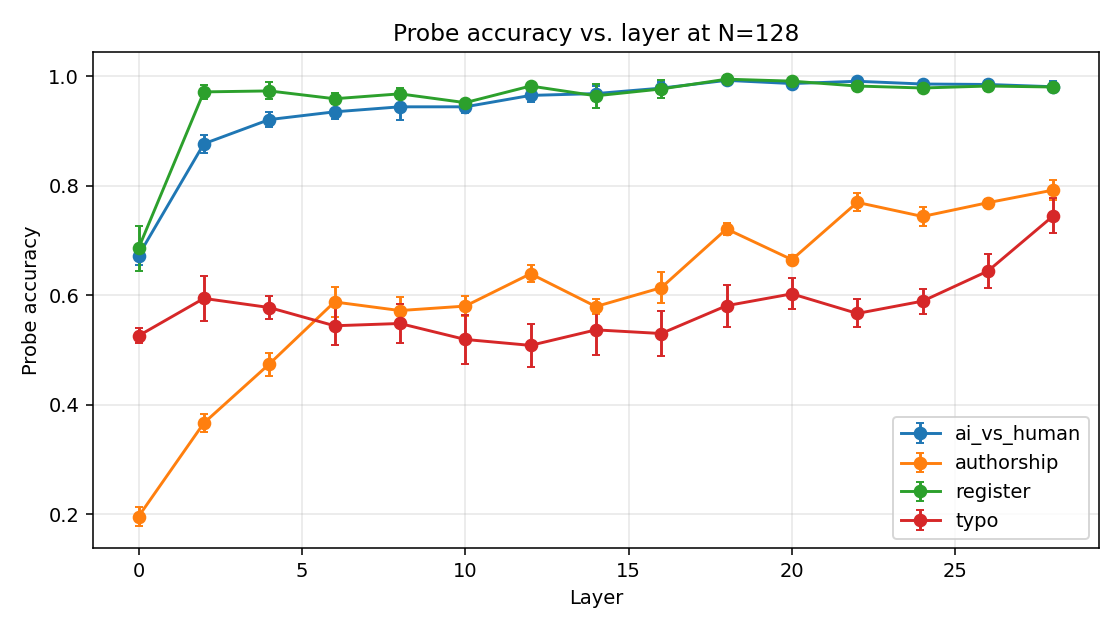
\includegraphics[width=0.95\linewidth]{figures/acc_vs_layer.png}
\caption{Probe accuracy as a function of layer for each \modes at $N=128$, averaged over 5 CV folds. \aihuman and \register climb sharply by layer 2 and saturate well before the final block. \authorship rises gradually across the entire stack and does not saturate. \typo is nearly flat through the middle layers and rises only at the very last layers, suggesting it is encoded in lexical-surface structure that becomes explicit only as the model prepares to emit tokens.}
\label{fig:layer}
\end{figure}

\begin{itemize}[leftmargin=*,itemsep=0pt,topsep=0pt]
\item \textbf{Shallow content \modes.} \aihuman and \register jump from $\sim$0.6 at the embedding layer to $\sim$0.95 by $L=2$ and saturate near 0.99 by $L=18$. Content/register cues are present in shallow distributional features and require no deep semantic integration.
\item \textbf{Gradual author \modes.} \authorship climbs monotonically from 0.20 ($L=0$) to 0.79 ($L=28$), with final layers still contributing. This matches the shape reported by \citet{sarfati2025prompt} for literary-author probing on \llama and supports the view that author identity is integrated from many lexical and syntactic cues across the whole stack.
\item \textbf{Late surface \modes.} \typo is essentially flat at $\sim$0.55 across middle layers, climbing only at the final layers to 0.74. The late layers are where the model commits to next-token distributions; surface-typing artifacts are visible there because that is where lexical-surface differences become read-out behaviour.
\end{itemize}

\Figref{fig:heatmaps} shows the full $N \times L$ heatmap per mode. \register saturates already at $N=32$, while \authorship shows the largest $N$-dependence, consistent with \citet{sarfati2025prompt}'s observation that 64--128 tokens are the sweet spot for stylometric probing.

\begin{figure}[t]
\centering
\begin{subfigure}[b]{0.24\textwidth}
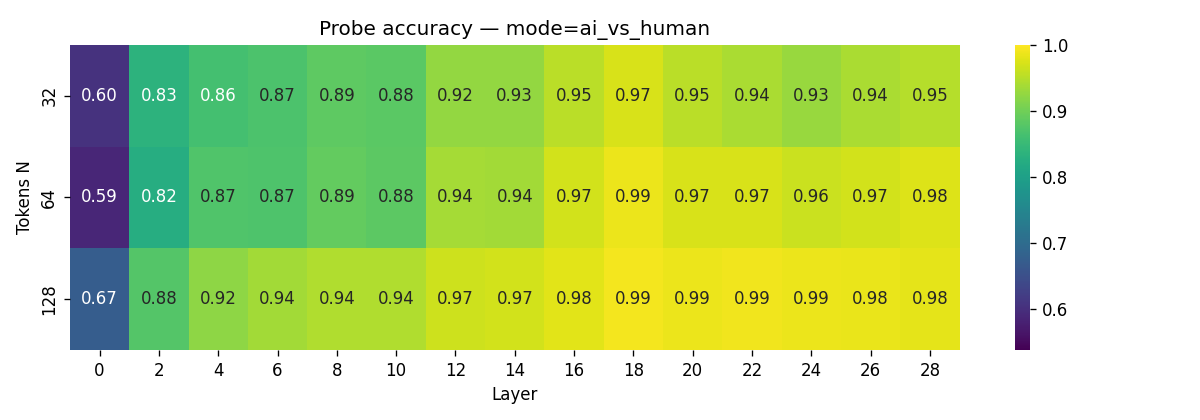
\includegraphics[width=\textwidth]{figures/heatmap_ai_vs_human.png}
\caption{\aihuman}
\label{fig:heat_ai}
\end{subfigure}
\begin{subfigure}[b]{0.24\textwidth}
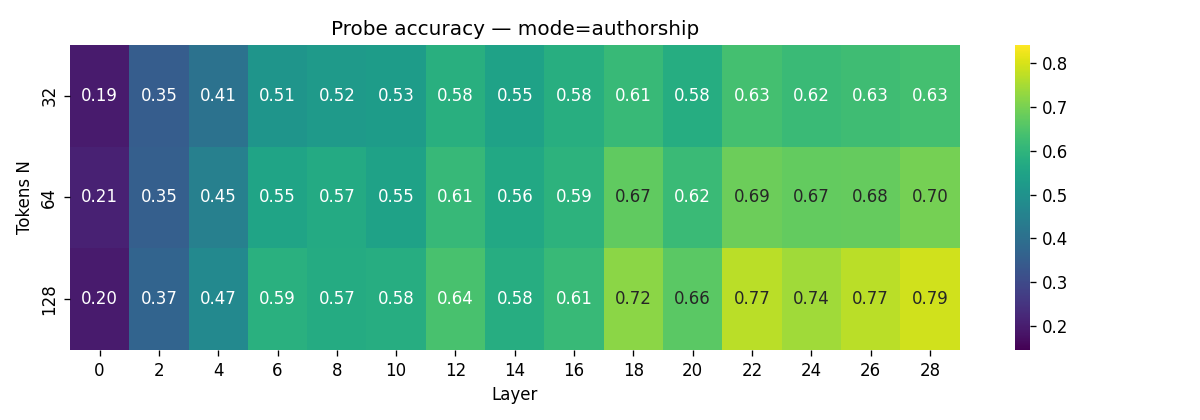
\includegraphics[width=\textwidth]{figures/heatmap_authorship.png}
\caption{\authorship}
\label{fig:heat_auth}
\end{subfigure}
\begin{subfigure}[b]{0.24\textwidth}
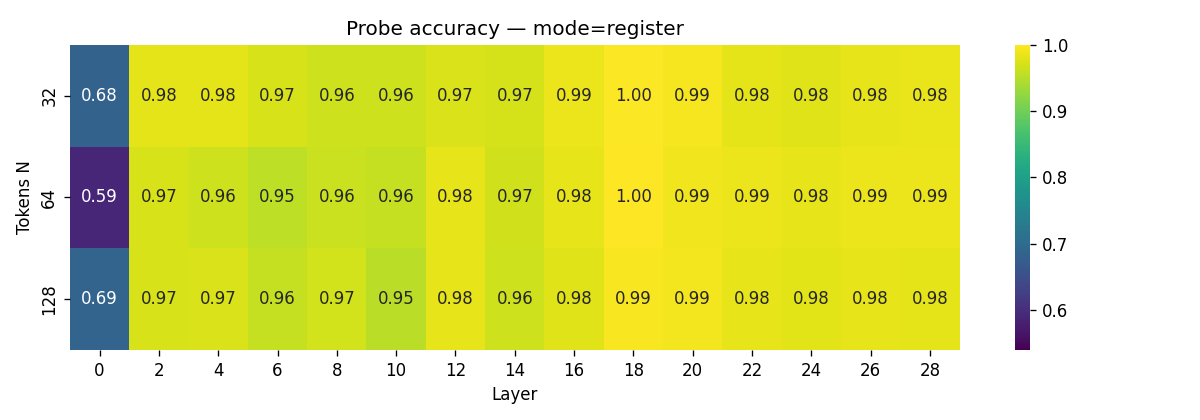
\includegraphics[width=\textwidth]{figures/heatmap_register.png}
\caption{\register}
\label{fig:heat_reg}
\end{subfigure}
\begin{subfigure}[b]{0.24\textwidth}
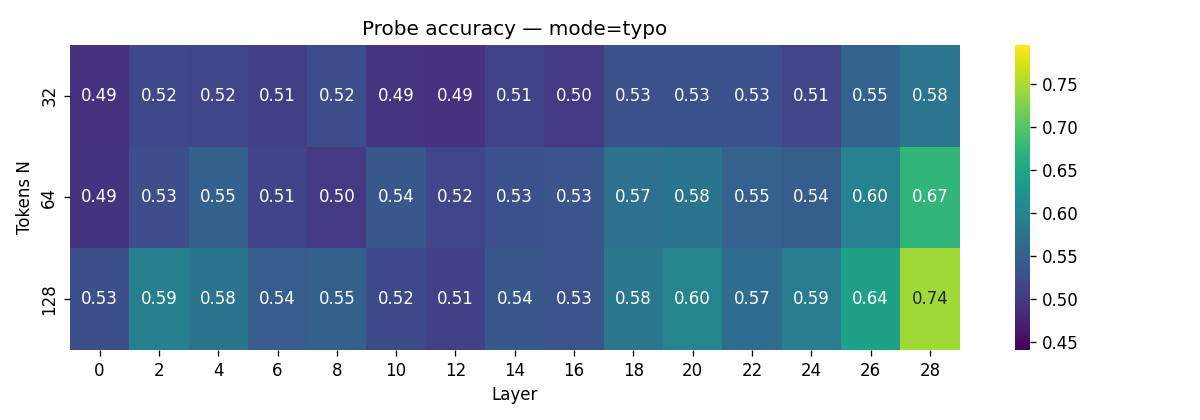
\includegraphics[width=\textwidth]{figures/heatmap_typo.png}
\caption{\typo}
\label{fig:heat_typo}
\end{subfigure}
\caption{Probe accuracy as a function of context length $N$ (rows) and layer $L$ (columns) for each \modes. \register saturates already at $N=32$; \authorship requires longer context; \typo is the only \modes for which gains are concentrated at the deepest layers.}
\label{fig:heatmaps}
\end{figure}

\subsection{Inter-mode geometry}
\label{sec:results-geom}

\para{Direction cosines.} \Tabref{tab:cosine} reports pairwise cosine similarities between probe directions at $L=28, N=128$. All six off-diagonal entries satisfy $|\cos| \leq 0.18$ --- \modes directions are pairwise near-orthogonal in the 1536-dimensional hidden space. The largest entry, \register $\leftrightarrow$ \authorship at 0.18, reflects the fact that 19th-century literary prose is overwhelmingly formal, so a formality direction has weak alignment with a Joyce-vs-Twain direction.

\begin{table}[t]
\centering
\caption{Pairwise cosine similarity between unit-normalized \modes directions at $L=28$, $N=128$. All off-diagonal entries satisfy $|\cos| \leq 0.18$.}
\label{tab:cosine}
\begin{tabular}{@{}lcccc@{}}
\toprule
 & \aihuman & \register & \typo & \authorship \\
\midrule
\aihuman    & 1.00 & $-0.04$ & 0.01 & $-0.04$ \\
\register   & $-0.04$ & 1.00 & 0.00 & 0.18 \\
\typo       & 0.01 & 0.00 & 1.00 & 0.00 \\
\authorship & $-0.04$ & 0.18 & 0.00 & 1.00 \\
\bottomrule
\end{tabular}
\end{table}

\para{Cross-mode probe transfer.} \Tabref{tab:transfer} reports the accuracy of a 1-D \logreg trained on the projection of mode-$B$ data onto mode-$A$'s probe direction. The picture has three components.

\begin{table}[t]
\centering
\caption{Cross-mode transfer accuracy. Cell $(A, B)$: train \logreg on the projection of mode-$B$ data onto mode-$A$'s probe direction; report 5-fold CV accuracy. Diagonals are the within-mode probe accuracy at $L=28$.}
\label{tab:transfer}
\begin{tabular}{@{}lccc@{}}
\toprule
\multirow{2}{*}{\textbf{Train direction (A)}} & \multicolumn{3}{c}{\textbf{Test mode (B)}} \\
\cmidrule(lr){2-4}
 & \aihuman & \register & \typo \\
\midrule
\aihuman   & 1.00 & 0.60 & 0.52 \\
\register  & \textbf{0.74} & 1.00 & 0.48 \\
\typo      & 0.62 & 0.50 & 1.00 \\
\bottomrule
\end{tabular}
\end{table}

\begin{itemize}[leftmargin=*,itemsep=0pt,topsep=0pt]
\item \textbf{One content-driven overlap.} The \register $\to$ \aihuman cell is 0.74 --- well above chance. Projecting AI-vs-human data onto the formality direction recovers three quarters of the AI-vs-human label. This is the latent footprint of ChatGPT's well-documented formality bias.
\item \textbf{Independent modes transfer at chance.} \register $\leftrightarrow$ \typo cells are 0.48 and 0.50 --- indistinguishable from chance. Synthetic keyboard-layout typo patterns share no direction with stylistic register, exactly as expected from independent generative processes.
\item \textbf{Weak typo $\to$ AI overlap.} \typo $\to$ \aihuman at 0.62 is modestly above chance, plausibly because typo-free machine-style text reads as more AI-like.
\end{itemize}

The cosine matrix and the transfer matrix tell a consistent story: production \modes are near-orthogonal directions in hidden state, and the overlaps that exist trace to identifiable content correlations rather than to a shared underlying axis.

\subsection{Probe vs.\ TF-IDF baseline}
\label{sec:results-baseline}

\Figref{fig:baseline} and \tabref{tab:baseline} compare neural-probe and \tfidf accuracies. The neural probe beats \tfidf by +10.9 points for \aihuman and is statistically tied on \register; \tfidf is stronger on \authorship and \typo.

\begin{figure}[t]
\centering
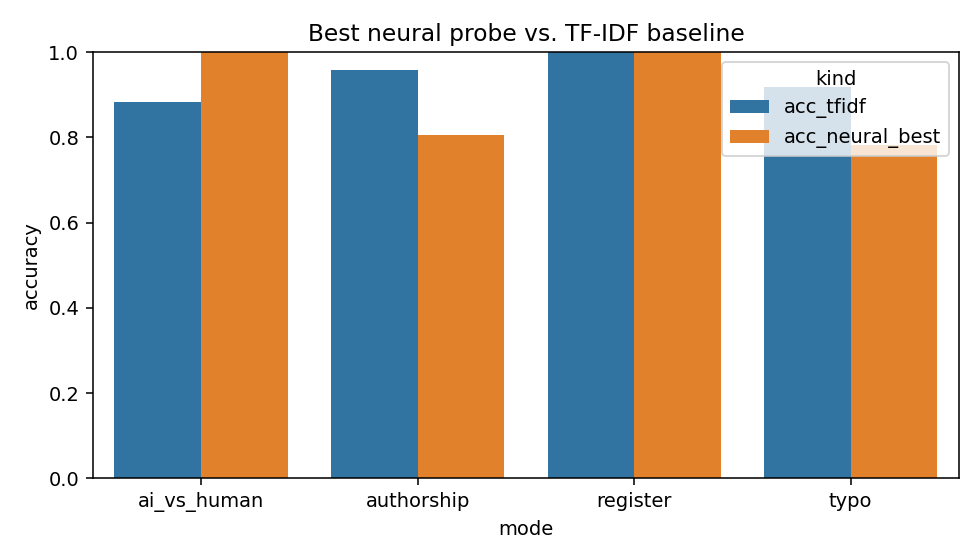
\includegraphics[width=0.7\linewidth]{figures/probe_vs_baseline.png}
\caption{Neural probe vs.\ \tfidf baseline. Surface n-grams dominate \modes whose signal is in explicit lexical form (\authorship, \typo); the neural probe dominates \modes whose signal requires distributional integration (\aihuman).}
\label{fig:baseline}
\end{figure}

\begin{table}[t]
\centering
\caption{Neural probe vs.\ \tfidf surface baseline. $\Delta$ is the probe$-$\tfidf gap. Best per row in \textbf{bold}.}
\label{tab:baseline}
\begin{tabular}{@{}lccc@{}}
\toprule
\textbf{Mode} & \textbf{TF-IDF} & \textbf{Probe} & \textbf{$\Delta$ (probe $-$ TF-IDF)} \\
\midrule
\aihuman    & 0.884 & \textbf{0.993} & $+0.109$ \increase \\
\authorship & \textbf{0.958} & 0.792 & $-0.166$ \decrease \\
\register   & \textbf{1.000} & 0.998 & $-0.002$ \pstar \\
\typo       & \textbf{0.919} & 0.745 & $-0.174$ \decrease \\
\bottomrule
\end{tabular}
\end{table}

The take-away is not that the neural probe is weaker. \tfidf has 20K explicit lexical features and trivially separates Joyce from Twain by vocabulary alone; it sees misspelled tokens as their own dimensions, while a 1536-dimensional hidden state has to integrate them. The neural probe accesses a different kind of representation. Its real interest is geometric --- the orthogonality and cross-mode transfer reported above are properties that \tfidf cannot exhibit because \tfidf has no shared representation space across \modes.

\subsection{Subspace geometry}

\Tabref{tab:dim} reports intrinsic dimensionality. Binary \modes have intrinsic dim 1 by construction. \authorship covers 95\% of inter-author variance with only 5 dimensions --- a 7-author corpus living in a 5-dim subspace of a 1536-dim residual stream, broadly consistent with \citet{sarfati2025prompt}'s $\sim$16-PCA result for 13 books. The first-PC variance of full-data restricted to each \modes (0.18--0.34) shows the \modes carve out non-trivial fractions of the embedding manifold.

\begin{table}[t]
\centering
\caption{Intrinsic dimensionality of each \modes subspace. ``Intrinsic dim'': number of PCs needed to explain 95\% of inter-class variance. ``1st-PC var'': variance explained by the first PC of all data restricted to the mode corpus.}
\label{tab:dim}
\begin{tabular}{@{}lccc@{}}
\toprule
\textbf{Mode} & \textbf{Classes} & \textbf{Intrinsic dim (95\%)} & \textbf{1st-PC var of full data} \\
\midrule
\aihuman    & 2 & 1 & 0.178 \\
\authorship & 7 & 5 & 0.336 \\
\register   & 2 & 1 & 0.212 \\
\typo       & 2 & 1 & 0.265 \\
\bottomrule
\end{tabular}
\end{table}

\subsection{Summary of evidence}

\Tabref{tab:hyp} summarises which sub-claims of the \modes hypothesis are supported by the experiments.

\begin{table}[t]
\centering
\caption{Verdict on each sub-claim of the production-\modes hypothesis. Evidence references the relevant tables and figures.}
\label{tab:hyp}
\begin{tabular}{@{}p{6cm}lp{6cm}@{}}
\toprule
\textbf{Sub-claim} & \textbf{Verdict} & \textbf{Evidence} \\
\midrule
H1. Each \modes decodable $>$75\% & Supported (4/4) & \Tabref{tab:main}: 0.745--0.998 \\
H2. Monotone climb with depth & Supported (3/4); \typo emerges only at deep layers & \Figref{fig:layer} \\
H3. Low intrinsic dim ($\lesssim 20$) & Supported & \Tabref{tab:dim}: all $\leq 5$ \\
H4. Pairwise near-orthogonal directions & Supported & \Tabref{tab:cosine}: max $|\cos| = 0.18$ \\
H5. Cross-mode transfer near chance except for content-correlated overlaps & Supported & \Tabref{tab:transfer}: only \register $\to$ \aihuman is well above chance \\
\bottomrule
\end{tabular}
\end{table}
